\documentclass[11pt,twocolumn]{article}

\usepackage{array}
\usepackage[url=false, doi=false]{biblatex}
\usepackage{booktabs}
\usepackage[font=footnotesize, labelfont=bf]{caption}
\usepackage{enumitem}
\usepackage[symbol]{footmisc}
\usepackage[scale=0.85]{geometry}
\usepackage{lipsum}
\usepackage{microtype}
\usepackage{multirow}
\usepackage{parskip}
\usepackage{siunitx}
\usepackage{titlesec}
\usepackage[dvipsnames]{xcolor}
\usepackage{xurl}
\usepackage[hidelinks]{hyperref}
\usepackage[nameinlink,capitalise]{cleveref}
\usepackage{verbatim}
\usepackage{graphicx}

\addbibresource{../bibliography.bib}

\titlelabel{}

\newcommand{\atom}[1]{\colorbox{Gray!30}{\ttfamily #1}}
\newcommand{\citen}[1]{~\parencite{#1}}
\newcommand{\citeay}[1]{\textcite{#1}}

\setcounter{footnote}{1}

\title{Using SAT features to guide Tableau provers \\[3pt] \large (possibly for AITP, hopefully for my first-year report)}
\date{}
\author{}

\begin{document}
\twocolumn[
	\centering
	\vspace{1em}
	{\LARGE\bfseries Using SAT features to guide Tableau provers \par} \vspace{3pt}
	{\large (possibly for AITP, hopefully for my first-year report) \par}
	\vspace{2em}
]
% \maketitle

\section{Introduction and Research}

\citeauthor{eliminatingModels} introduce SATCoP\citen{eliminatingModels}, a tableau prover based on LeanCoP\citen{Otten2023leanCoP20} that runs a separate SAT solver along fed with grounded atoms from the tableau prover.
If the SAT solver reaches an unsatisfiable state, then we can prove that the entire tree is unsatisfiable.

This approach is sound, but incomplete.
There are many problems that cannot be directly proven by this combination.

\section{Novel Idea}

Besides saying whether the current prover is UNSAT, CaDiCaL\citen{cadical20} gives us extra information.
\begin{description}[style=nextline]
	\item[\atom{probe\_conflicts}] For every SAT literal $a$, will $\neg a$ cause UNSAT?
	\item[\atom{forced\_true}] Is this candidate subgoal forced true by the SAT solver?
	\item[\atom{evsids}] Sum of EVSIDS scores for all grounded atoms of a certain formula.
	\item[\atom{subgoal\_count}] Number of remaining subgoals introduced by the extension (lower is better). This is similar to one of the heuristics used by \citeay{letzModelEliminationConnection2001}.
\end{description}

\section{Implementation}

I create a strategy, \atom{SATSolveGuided}, which chooses the start, extension, or reduction with the highest one of these properties.
It prefers starts first, reductions later, and extensions only of none of these two are presents.

However, experimentation showed that calculating these properties for all leafs is slow.
% Codex: if there is only one start/extension/reduction then none of these are calculated, right?
For this reason I experiment with 6 different strategies.
\begin{description}[style=nextline]
	\item[SATSolveGuided] \atom{(probe\_conflicts, forced\_true,} \\ \atom{evsids, -subgoal\_count)}
	\item[SATSolveGuidedProbeConflicts] \atom{(probe\_conflicts)}
	\item[SATSolveGuidedForcedTrue] \atom{(forced\_true)}
	\item[SATSolveGuidedEVSIDS] \atom{(evsids)}
	\item[SATSolveGuidedShort] \atom{(-subgoal\_count)}
	\item[SATSolveGuidedFast] \atom{(forced\_true, evsids, -subgoal\_count)}
\end{description}

I use the existing connection prover implementation as a base for this code\citen{connections_2023}.
This allows me to use the existing code for hard things like Prolog parsing, and also to use PyCoP as a control group.

\section{Results}

\begin{figure}[h]
	\centering
	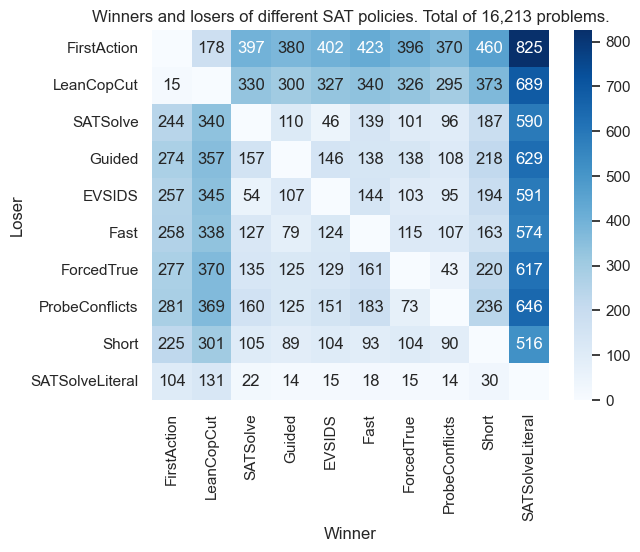
\includegraphics[width=\columnwidth]{../../figures/sat_policies_plot.png}
	\caption{Winners and losers of different SAT policies in a subset of 1458 problems\citen{chvalovsky2021characteristic}. I expect these percentages to be similar in the whole set.}
\end{figure}

\newcommand{\MS}{{\color{BrickRed}\bfseries max-steps}}
\newcommand{\TO}{{\color{OrangeRed}\bfseries timeout}}
\newcommand{\best}{\color{Green}}

\sisetup{
    table-format = 11.0,
	table-text-alignment = right,
}

\setlength{\defaultaddspace}{4pt}

Experiments were run on the University of Cambridge CSD3 Ice Lake cluster, using one node per experiment with 76 physical CPU cores and 256 GiB RAM.

\begin{table*}[t]
      \centering
      \scriptsize
      \begin{tabular}{@{}>{\ttfamily\bfseries}l l r S[table-format=5.0] S[table-format=6.0]@{}}
          \toprule
          {\rmfamily\bfseries Problem} & {\bfseries Strategy} & {\bfseries Solved} & {\bfseries Steps} & {\bfseries Time (ms)} \\
          \midrule
          \multirow{7}{*}{KRS255+1.p}
              & \atom{SATSolve}                     & \texttt{false}  & 12659 & 90003 \\
              & \atom{SATSolveGuided}               & \texttt{false}  &  9104 & 90002 \\
              & \atom{SATSolveGuidedProbeConflicts} & \texttt{false}  & 10533 & 90002 \\
              & \atom{SATSolveGuidedForcedTrue}     & \texttt{true} &  7423 & 40270 \\
              & \atom{SATSolveGuidedEVSIDS}         & \texttt{true} &  6516 & 39185 \\
              & \atom{SATSolveGuidedShort}          & \texttt{false}  & 13201 & 90007 \\
              & \atom{SATSolveGuidedFast}           & \texttt{false}  & 12547 & 90011 \\
          \addlinespace

          \multirow{7}{*}{GEO214+2.p}
              & \atom{SATSolve}                     & \texttt{false}  & 24308 & 90001 \\
              & \atom{SATSolveGuided}               & \texttt{true} &  4831 &  4622 \\
              & \atom{SATSolveGuidedProbeConflicts} & \texttt{false}  & 90966 & 90000 \\
              & \atom{SATSolveGuidedForcedTrue}     & \texttt{false}  & 93502 & 90000 \\
              & \atom{SATSolveGuidedEVSIDS}         & \texttt{false}  & 24030 & 90013 \\
              & \atom{SATSolveGuidedShort}          & \texttt{true} & 15944 & 34071 \\
              & \atom{SATSolveGuidedFast}           & \texttt{true} &  4440 &  3816 \\
          \addlinespace

          \multirow{7}{*}{SYN578-1.p}
              & \atom{SATSolve}                     & \texttt{false}  & {--}  & {--} \\
              & \atom{SATSolveGuided}               & \texttt{true} & 21388 & 103259 \\
              & \atom{SATSolveGuidedProbeConflicts} & \texttt{true} & 11347 &  33783 \\
              & \atom{SATSolveGuidedForcedTrue}     & \texttt{true} & 11994 &  32949 \\
              & \atom{SATSolveGuidedEVSIDS}         & \texttt{false}  & {--}  & {--} \\
              & \atom{SATSolveGuidedShort}          & \texttt{true} & 25291 & 100802 \\
              & \atom{SATSolveGuidedFast}           & \texttt{true} & 11083 &  22460 \\
          \addlinespace

          \multirow{7}{*}{SYN583-1.p}
              & \atom{SATSolve}                     & \texttt{false}  & {--}  & {--} \\
              & \atom{SATSolveGuided}               & \texttt{true} & 13439 & 50791 \\
              & \atom{SATSolveGuidedProbeConflicts} & \texttt{false}  & {--}  & {--} \\
              & \atom{SATSolveGuidedForcedTrue}     & \texttt{false}  & {--}  & {--} \\
              & \atom{SATSolveGuidedEVSIDS}         & \texttt{true} & 12521 & 46118 \\
              & \atom{SATSolveGuidedShort}          & \texttt{true} & 13723 & 52979 \\
              & \atom{SATSolveGuidedFast}           & \texttt{true} & 11991 & 37213 \\
          \addlinespace

          \multirow{7}{*}{SYN657-1.p}
              & \atom{SATSolve}                     & \texttt{false}  & {--}  & {--} \\
              & \atom{SATSolveGuided}               & \texttt{true} & 10996 & 60140 \\
              & \atom{SATSolveGuidedProbeConflicts} & \texttt{false}  & {--}  & {--} \\
              & \atom{SATSolveGuidedForcedTrue}     & \texttt{false}  & {--}  & {--} \\
              & \atom{SATSolveGuidedEVSIDS}         & \texttt{false}  & {--}  & {--} \\
              & \atom{SATSolveGuidedShort}          & \texttt{false}  & {--}  & {--} \\
              & \atom{SATSolveGuidedFast}           & \texttt{false}  & {--}  & {--} \\
          \bottomrule
      \end{tabular}
      \caption{Some random problems solved by different SAT-guided strategies, as a representative example}
      \label{tab:sat-guided-problems}
  \end{table*}

% A subset of 247 ``representative'' TPTP problems was used for evaluation\citen{chvalovsky2021characteristic}.
% The results with any significance are found in \cref{big_table}.
% 
% The comparer runs all 6 policies in parallel, with a 30-second time limit and a \num{50000} step limit.
% A larger experiment, with the entirety of TPTP and a longer time limit, will come in the future.
% 
% I also post-process the canonical TPTP runs into short serial schedules.
% For each strategy and time cap, the pair ``strategy + cap'' is treated as covering exactly the problems that the strategy solves within that cap.
% The schedule synthesis problem is therefore a budgeted maximum-coverage problem with a multiple-choice knapsack constraint: choose at most one cap per strategy, subject to a global budget of 60 or 120 seconds, and maximise either the total number of solved problems or the number of solved problems outside LeanCopCut's solved set.
% After fixing the capped strategies, I then order them by a second optimisation pass that minimises total runtime over the benchmark set, using the recorded per-problem runtimes and charging the full cap on timeout rows.
% 
% The results show that all three policies have marked improvements in certain problems.
% It's likely that with further exploration we might get even better results than the control groups.

\renewcommand*{\bibfont}{\small}
\printbibliography{}

\end{document}
